%% LyX 1.6.2 created this file.  For more info, see http://www.lyx.org/.
%% Do not edit unless you really know what you are doing.
\documentclass[conference,english]{IEEEtran}
\usepackage[T1]{fontenc}
\usepackage[latin9]{inputenc}
\usepackage{babel}

\usepackage{float}
\usepackage{textcomp}
\usepackage{amsthm}
\usepackage{amsmath}
\usepackage{graphicx}
\usepackage[unicode=true, pdfusetitle,
 bookmarks=true,bookmarksnumbered=false,bookmarksopen=false,
 breaklinks=false,pdfborder={0 0 1},backref=false,colorlinks=false]
 {hyperref}

\makeatletter

%%%%%%%%%%%%%%%%%%%%%%%%%%%%%% LyX specific LaTeX commands.
\newcommand{\noun}[1]{\textsc{#1}}
%% Because html converters don't know tabularnewline
\providecommand{\tabularnewline}{\\}
\floatstyle{ruled}
\newfloat{algorithm}{tbp}{loa}
\floatname{algorithm}{Algorithm}

%%%%%%%%%%%%%%%%%%%%%%%%%%%%%% Textclass specific LaTeX commands.
\theoremstyle{plain}
\newenvironment{lyxcode}
{\par\begin{list}{}{
\setlength{\rightmargin}{\leftmargin}
\setlength{\listparindent}{0pt}% needed for AMS classes
\raggedright
\setlength{\itemsep}{0pt}
\setlength{\parsep}{0pt}
\normalfont\ttfamily}%
 \item[]}
{\end{list}}

\@ifundefined{showcaptionsetup}{}{%
 \PassOptionsToPackage{caption=false}{subfig}}
\usepackage{subfig}
\makeatother

\begin{document}

\title{Using Python in Computer Vision:\\ Performance and Usability}

\author{\IEEEauthorblockN{Brian Thorne, Rapha�l Grasset}
\IEEEauthorblockA{HIT Lab NZ\\
University of Canterbury\\
Private Bag 4800, Christchurch\\
Email: brian.thorne@hitlabnz.org,raphael.grasset@hitlabnz.org}
\and
\IEEEauthorblockN{Richard Green}
\IEEEauthorblockA{Computer Science and Software Engineering\\
University of Canterbury\\
Private Bag 4800, Christchurch\\
Email: richard.green@canterbury.ac.nz}}

\maketitle
\begin{abstract}
Python is a popular language widely used by the scientific community
due to its clear syntax and an extensive number of specialized packages.
For image processing or computer vision development, two libraries
are prominently used: \textit{NumPy/SciPy} and \textit{OpenCV} with the Python Wrapper. In this paper, we present a comparative evaluation
of both libraries, assessing their performance as well as their usability. We also describe our results regarding the performance of python wrapper vs native C implementation of OpenCV.\end{abstract}
\begin{keywords}
Computer Vision, Python, SciPy, OpenCV
\end{keywords}

\section{Introduction}

Python\cite{van1994python} has been of growing interest to the academic
community over the last decade, widely used by the computational science community. 
The simple syntax of Python, high level dynamic data types, and automated memory management has driven their attention 
and forged it as a popular tool for the research community.

The field of image processing and computer vision (CV)
has been driven for the last decade by development in C/C++ and the
usage of the MATLAB software \cite{kovesi-matlab}. Although MATLAB offers an efficient
high level platform for prototyping and testing algorithms, its performances
doesn't compete with a well designed and optimized C/C++ implementation.
More recently, we have seen the emergence of potential and valuable
solutions for developing image processing and computer vision algorithms
in Python.

The goal of this paper is to evaluate the performances and usability of the most common
solutions for developing CV algorithms and CV applications in Python. Indeed, we aim to offer a comprehensive
overview of the advantages/disadvantages of using Python for computer vision development that can be beneficial
for any scholar intrigued by the topic.

We have focused our attention on the performances of two widely used
CV libraries in Python: \textit{OpenCV} \cite{bradski2000opencv} and
\textit{NumPy/SciPy} \cite{oliphant2007python}. For this matter, we
analyzed their performances through a list of common tasks and processes
regularly employed in computer vision (e.g. video capture, filtering
algorithms, feature detection, etc). We were particularly interested
to learn how Python performs in comparison with the native C implementation
of OpenCV considering the low level calling of the original OpenCV C functions.

After an introduction of our experimental process, we will describe successively
the tests employed and the results we obtained, before finally discuss our
findings and provide recommendations.


\section{Experimental Process}

In this section, we briefly introduce the different libraries we tested
as our experimental apparatus and protocol.  

\subsection*{Libraries}

\textit{Python}. Python is a general purpose dynamic programming language \cite{entry-0}.
It is highly regarded due in no small part for its fast development
time and the ease of integrating packages \cite{sanner1999python}.
Python's performance makes it a viable programming language for scientific
work \cite{cai2005performance}, and it has also been used members in the
CV community for many years \cite{doakPyCV}.
\\
\\
\textit{OpenCV}. Originally an Intel research initiative, \textit{OpenCV} is a cross-platform
open source computer vision library widely used for real time image
processing. It aims to provide well tested, optimized and open source
implementation of state of the artimage processing and computer vision algorithms.

The library is written in C, ensuring fast and portable code
(optionally to embedded platforms). The library is built above a core image library, which supports
image structure and basic image manipulation. This core image library has two forms: a software
implementation is provided freely whilst an accelerated version utilizing
the \textit{Integrated Performance Primitives} \cite{taylor2004intel}
can be optionally acquired from Intel. This latter option takes advantage
of the extended multimedia instructions set available on Intel Processors (e.g. SSE3, SSE4).

Nowadays, multiple language bindings are available for OpenCV, such
as OpenCVDotNet and EmguCV. Additional tools such as GPUCV \cite{farrugia2006gpucv}
have been made for OpenCV using graphics hardware to accelerate CV
performance. Multiple bindings to OpenCV such as OpenCV Python, and
PyCV \cite{tri2009principled} have been created for Python, as well
as the automatically built wrapped bindings based on SWIG \cite{beazley1996swig}
which we tested in this paper.
\\
\\
\textit{NumPy/SciPy}. \emph{NumPy} gives strongly typed N-dimensional array support to Python \cite{oliphant2006guide}.
It's a well recognized library, offering an easier approach for multidimensional
array manipulation than in the C programming language. A large part of 
the low level algorithms are implemented in C and FORTRAN (and wrapped around Python), resulting in very fast and optimized raw data crunching and iterating.

\emph{SciPy} \cite{jones2001scipy} is a set of Python libraries and
tools for scientific and mathematical work built on top of NumPy \cite{oliphant2007python}.
SciPy offers many different modules including routines such as numerical
integration, optimization, signal processing and image processing/computer vision functions. Two major tools are usually distributed
with SciPy that and very useful for computer vision development: Matplotlib and IPython.
Matplotlib \cite{hunter2007matplotlib} is an array and image plotting
library, and IPython \cite{perez2007ipython} is an improved interactive
shell for Python.

\subsection*{Apparatus}

We conducted our test on a Intel Core 2 Duo 6600 machine, with 3.8
RAM, running Ubuntu 9.04. 

For the test we compared these different libraries (all builds were 32-bit version): 
\begin{itemize}
\item OpenCV Native Language (OPENCV\_C): we used snapshot built version
1.1.1, rev 1978. The code has been compiled with the GNU tool chain
version (4.3.3), and in Release mode with O3 compiler optimizations,
MMX, fast math, SSE3. All additional packages, EXCEPT 1393, are turned
on (png, jpg, gtk, gstreamer, unicap, V4L). 
\item OpenCV Python Wrapper (OPENCV\_PY): we used the SWIG \cite{beazley1996swig}
wrapper version 1.3.36. We used a similar OpenCV build as the previous one.
\item SciPy/NumPy (SCIPY): we used the stable versions from the Ubuntu repositories:
SciPy version 0.7.0 and NumPy 1.2.1
\end{itemize}
 
For the camera, we conducted our test with an USB webcam, a BRIAN TO COMPLETE. White balance, focus and exposure have been fixed to a constant value a prior the tests. The test environment was a large room with 
neon lamps at the ceiling and a low amount of ambient light.

\subsection*{Evaluation Protocol}
For our testing, we cover different standard algorithms traditionally used in a CV applications as some major process relevant to computer vision (e.g. image acquisition). Our tests were aiming to reproduce general high level processes implied during CV applications development rather than low level function calls. 

For each of the tests we describe the
process, the difference in terms of syntax between the different libraries, the performance and the usability of each libraries. As we aims to provide implementation of the tests for the 3 tested libraries, some of the tests only focused comparing Python
OPENCV\_PY vs SCIPY. 
Reader can access the source code from the project website
\footnote{\href{http://code.google.com/p/pycam/wiki/PythonComputerVision}{http://code.google.com/p/pycam/wiki/PythonComputerVision}.}

\section{Quantitative Tests}

\subsection{Image Acquisition}

Live Image acquisition is largely utilized in a majority of CV applications.
We thus tested, frame acquisition and frame display as a first test. Added to performance results, we describe in this section the syntax between the different libraries for implementing this test.

\subsubsection*{Acquiring and displaying an image in C with OpenCV}

Algorithm \ref{alg:C-Image-capture} describes how to open up a new camera capture
device, capture one frame, open a new window and display the result%
\footnote{For presentation brevity we omitted in this paper the source code for error checking, cleanup and optimization. However they are present in the source code of our tests%
}. 

%Using this as a template it is straight forward to wrap the capture
%and display in a loop, this forms the basis of the C++ class \noun{VideoCapturePlayer}
%used in the other tests to keep the code duplication and variation
%in timing to an absolute minimum.

%
\begin{algorithm}[h]
\begin{lyxcode}
\#include~\textquotedbl{}cv.h\textquotedbl{}

\#include~\textquotedbl{}highgui.h\textquotedbl{}

int~main()\{

~~IplImage~~{*}frame;

~~CvCapture~{*}capture;

~~capture~=~cvCreateCameraCapture(0);

~~cvNamedWindow(~\textquotedbl{}Snapshot\textquotedbl{},~0~);

~~frame~=~cvQueryFrame(~capture~);

~~cvShowImage(~\textquotedbl{}Snapshot\textquotedbl{},~frame~);

\}
\end{lyxcode}
\caption{\label{alg:C-Image-capture}Image capture and display with OpenCV
in C}

\end{algorithm}



\subsubsection*{Acquiring and displaying an image in Python with OpenCV}

Algorithm \ref{alg:Python-Image-capture} show the equivalent through the python wrapper.
You can observe a high level of similarity with the previous version.
 main difference being in the Python code no variables types are declared. 

%
\begin{algorithm}[h]
\begin{lyxcode}
from~opencv~import~highgui~as~hg

capture~=~hg.cvCreateCameraCapture(0)

hg.cvNamedWindow(\textquotedbl{}Snapshot\textquotedbl{})

frame~=~hg.cvQueryFrame(capture)

hg.cvShowImage(\textquotedbl{}Snapshot\textquotedbl{},~frame)
\end{lyxcode}
\caption{\label{alg:Python-Image-capture}Image capture and display with OpenCV in Python}

\end{algorithm}
%
\begin{figure}[h]
\centering{}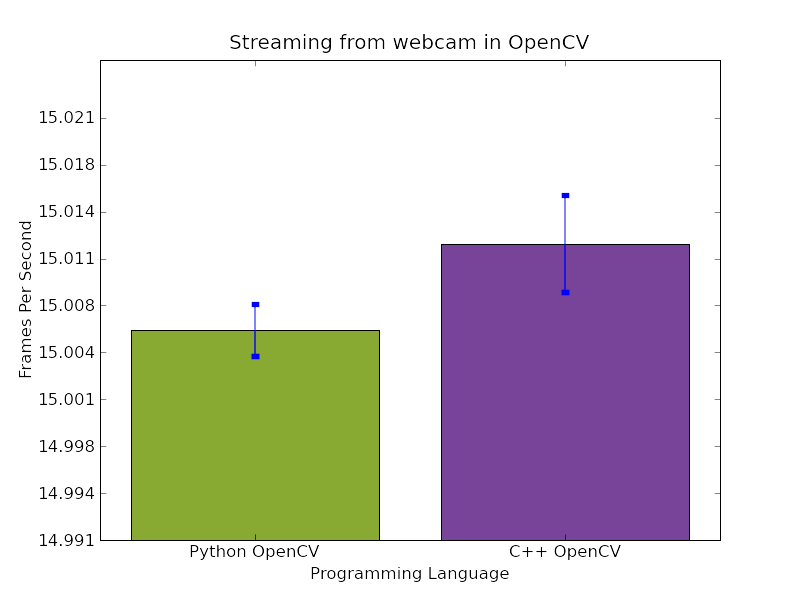
\includegraphics[width=0.95\columnwidth]{report_data/streaming_from_webcam_in_opencv}\caption{\label{fig:Streaming-comparison}Comparison of capture performances between OPENCV\_C, OPENCV\_PY (processing time).}

\end{figure}

\subsubsection*{Comparison}

Figure \ref{fig:Streaming-comparison} shows the performance results for
the previous algorithms. The measurement was done over a 2 minutes period for 3 iterations, averaging
the resulting frame rates. Python and C++ perform at very similar rates whilst carrying
out an I/O bound task. C++ having a marginally higher frame rate output
than Python. 

The SciPy package does not currently have a direct method for image capture, so we couldn't compare live acquisition.
However, we developed a solution for converting OpenCV camera capture to SciPy: after converting the image data to a NumPy arrays, we achieved that by creating and using a Python decorator which converts the image data before and after calling a Python function that processes on a NumPy image. A 640x480 RGB image takes less than 2ms to convert either way on the testing platform used throughout this report.

\subsection{Image Blur}

One of the simplest operations in image processing is blurring an
image. As this can be achieved in different ways, we focused here to test a basic
Gaussian blur. As well know, this is easily achieved by convolving
the image with a Gaussian filter. Because of the separability of multidimensional
Gaussian filters \cite{young1995recursive}, the convolution can be
applied in two ways; applying a 1 dimensional filter twice, once in
each direction; or secondly the image can be convolved with a 2-dimensional
Gaussian filter created by the product of two 1 dimensional filters.

Equation \ref{eq:1D Gaussian Filter} shows the Gaussian function
for obtaining the filter in one dimension and Equation \ref{eq:2D Gaussian Filter} shows the 2 dimensional case \cite{SS01}.
 \begin{equation}
G\left(x\right)=\frac{1}{\sqrt{2\pi}\sigma}e^{-\frac{x^{2}}{2\sigma^{2}}}\label{eq:1D Gaussian Filter}\end{equation}
\begin{equation}
G\left(x,y\right)=\frac{1}{\sqrt{2\pi}\sigma^{2}}e^{-\frac{x^{2}+y^{2}}{2\sigma^{2}}}\label{eq:2D Gaussian Filter}\end{equation}
with \textit{Sigma} the standard deviation of the Gaussian distribution. 

OpenCV includes a Gaussian filter implementation that can be applied to an image by calling
the \emph{\noun{cvSmooth}} function and passing the desired filter
size. SciPy has a n-dimensional Gaussian filter that acts on a NumPy
array. Both libraries use the 1 dimensional case, as it requires less
computation.

\begin{figure}[htbp]
\begin{centering}
\subfloat[OPENCV\_C]{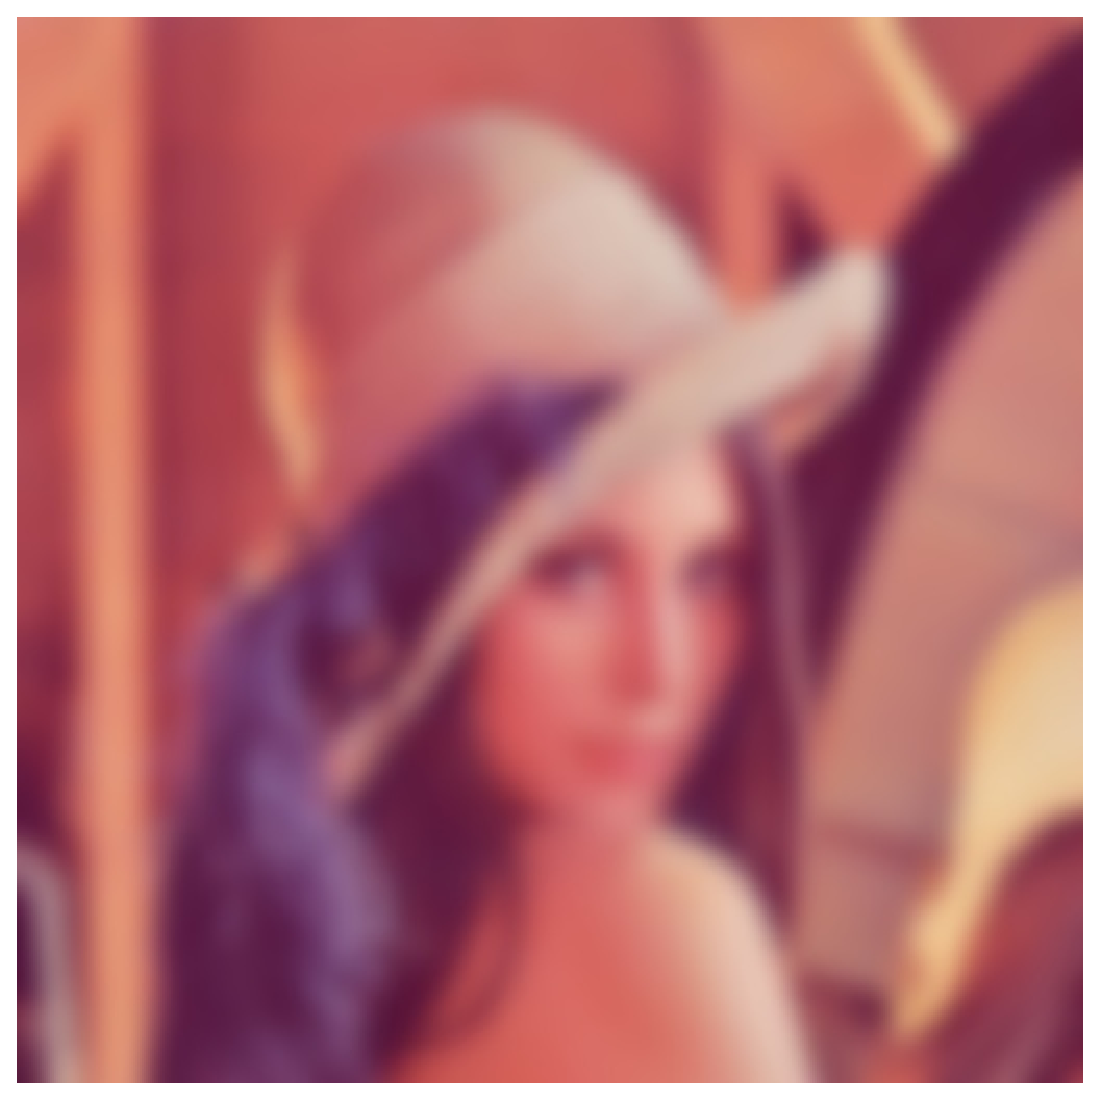
\includegraphics[width=0.33\columnwidth]{report_data/blurred_imag_cpp_opencv_gaussian}

}\subfloat[OPENCV\_PY]{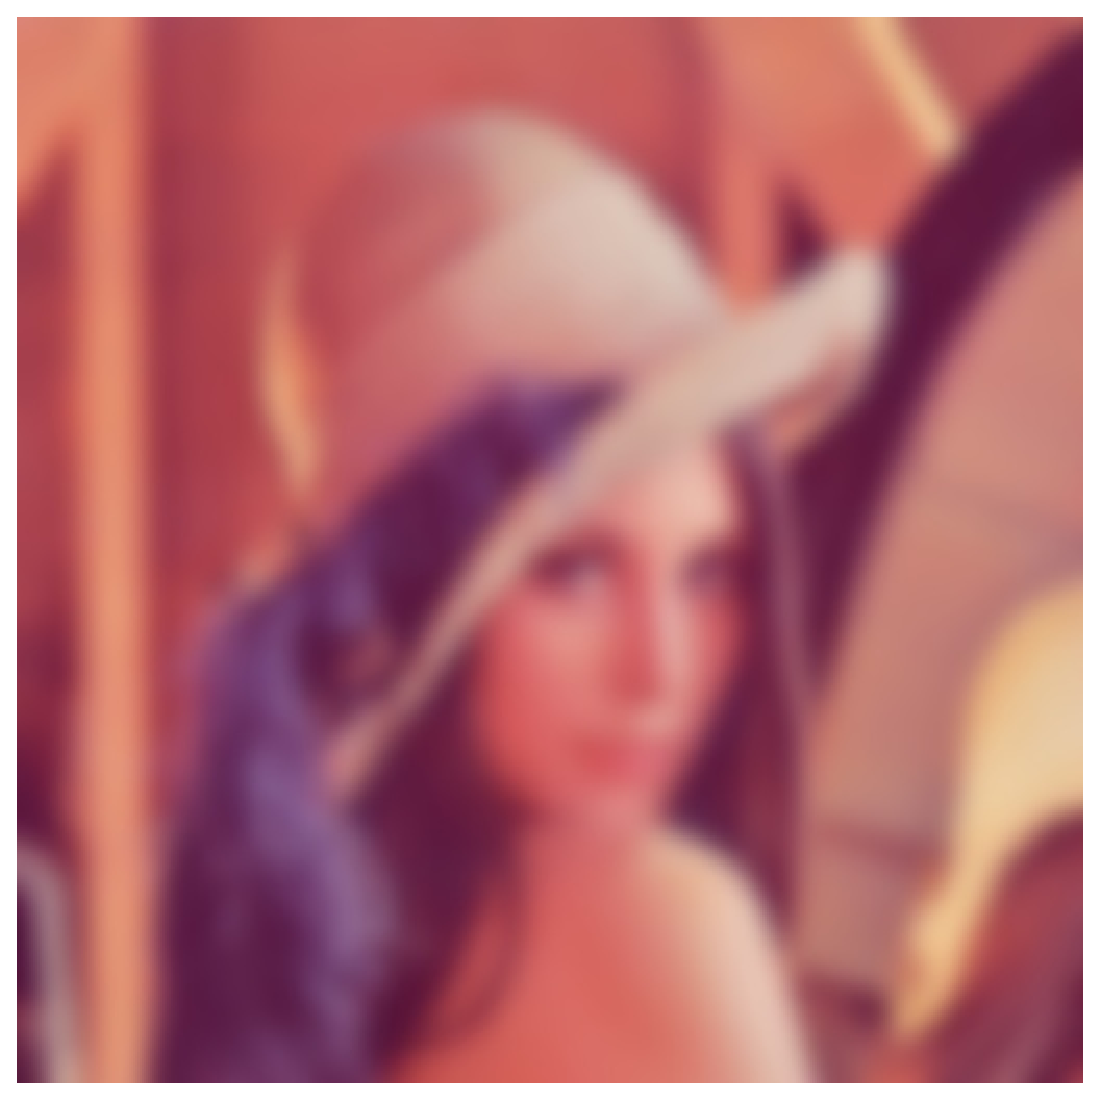
\includegraphics[width=0.33\columnwidth]{report_data/blurred_imag_python_opencv_gaussian}

}\subfloat[SCIPY]{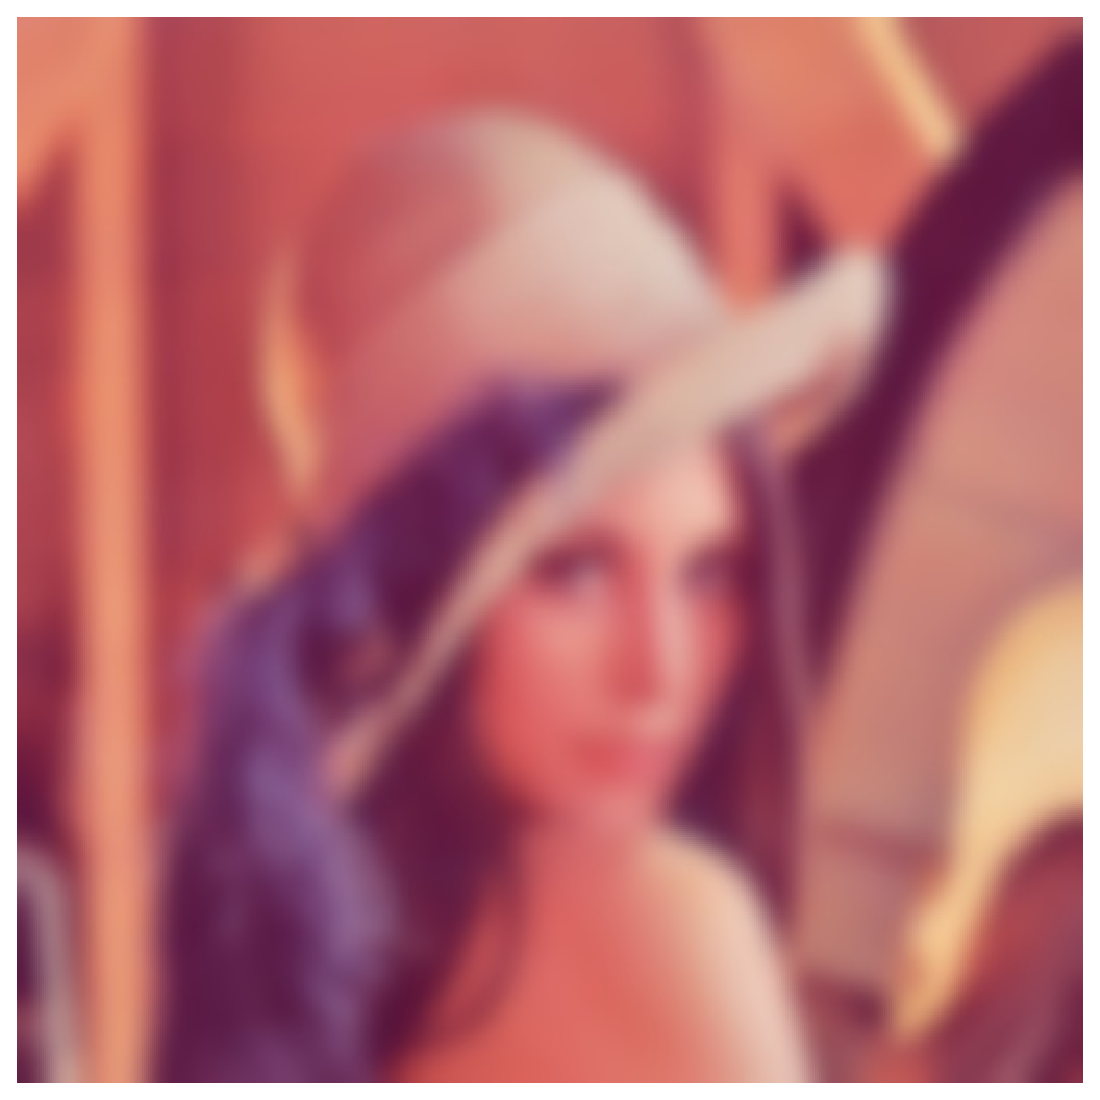
\includegraphics[width=0.33\columnwidth]{report_data/blurred_imag_python_scipy_gaussian}

}
\par\end{centering}

\caption{\label{fig:Gaussian-Output-Images}Generated Images from Gaussian Blur filter using OPENCV\_C, OPENCV\_PY and SCIPY on Lena dataset.}

\end{figure}

To ensure the same level of filtering is carried out for all the libraries, the filter parameters have been converted to be compatible with OpenCV's \noun{cvSmooth} defaults \cite{bradski2008learning}.

\subsubsection*{Comparison}

The blurred output images are shown on the Lena dataset in Figure \ref{fig:Gaussian-Output-Images}.
A basic image difference between confirmed similar results between C++/Python OpenCV version (as expected), but
small difference between SciPy and OpenCV Python code as presented Figure \ref{fig:Difference-of-each}. The graph in Figure \ref{fig:Difference-of-each} shows the pixel by pixel differences in each of the colour channels of a single image.
The maximim intensity difference at any point was 7.8\%, the mean difference was 0.8\% of the full intensity scale. 
%We obtained maximum intensity difference of 20, with an average difference of 2.1 with a standard deviation of 1.4.

\begin{figure}[htbp]
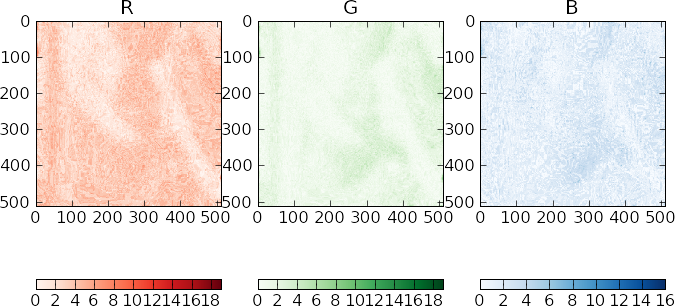
\includegraphics[width=0.98\columnwidth]{report_data/gaussian_diffs}
\caption{\label{fig:Difference-of-each} Channel Difference (RGB, 255 bits resolution) from Gaussian blur filter between OPENCV\_PY and SCIPY.}

\end{figure}

This could be simply explained by a potential difference in the implementation of the
Gaussian kernel approximations. In SciPy the filter is created by
a direct sampling of the Gaussian function; OpenCV on the other hand,
uses the size of the filter, this is a good indication it probably
uses the pascal triangle as an approximation for the Gaussian kernel \cite{ben1991image}.
These differences are minor, but it is worth noting that such a simple Gaussian blur provide such a different results.

%
\begin{figure}[htbp]
\begin{centering}
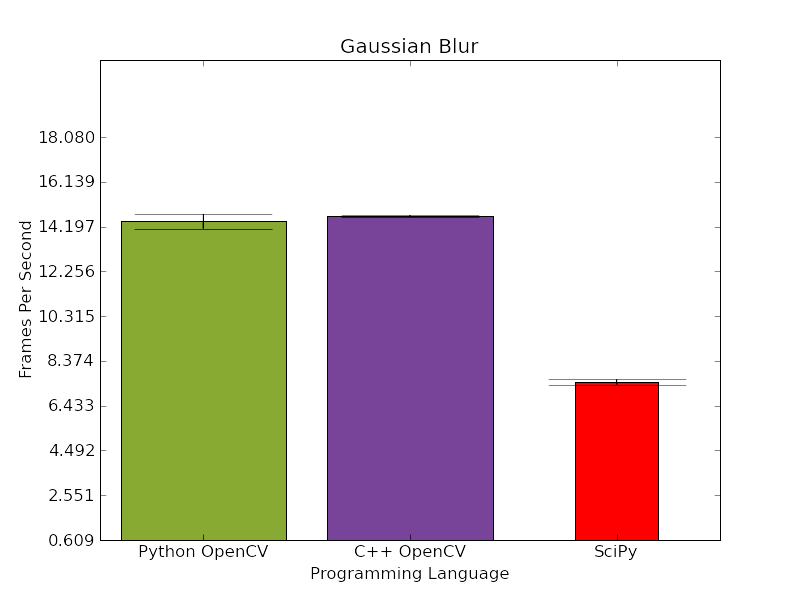
\includegraphics[width=0.9\columnwidth]{report_data/gaussian_blur}
\par\end{centering}

\caption{\label{fig:performance-gaussian}Comparison of gaussian blur performances between OPENCV\_C, OPENCV\_PY and SCIPY (processing time).}
\end{figure}

\subsection{Background subtraction}

A common task in security surveillance, human computer interaction is the detection of any visual changes in a video. This is done in its simplest form by a comparison of one frame to another previous frame \cite{gao2006robust}.
If the difference image is more than a certain threshold, something
has changed. An example is presented in Figure \ref{fig:Adding-a-single}
after adding a cellphone to a scene for the \noun{OPENCV\_PY} implementation.

As Figure \ref{fig:BackgroundSubtract_graph} shows, the performance
is very close for Python and C++ versions using OpenCV. Python was
faster on average, but the performance was more consistent in C++. 

%
\begin{figure}[htbp]
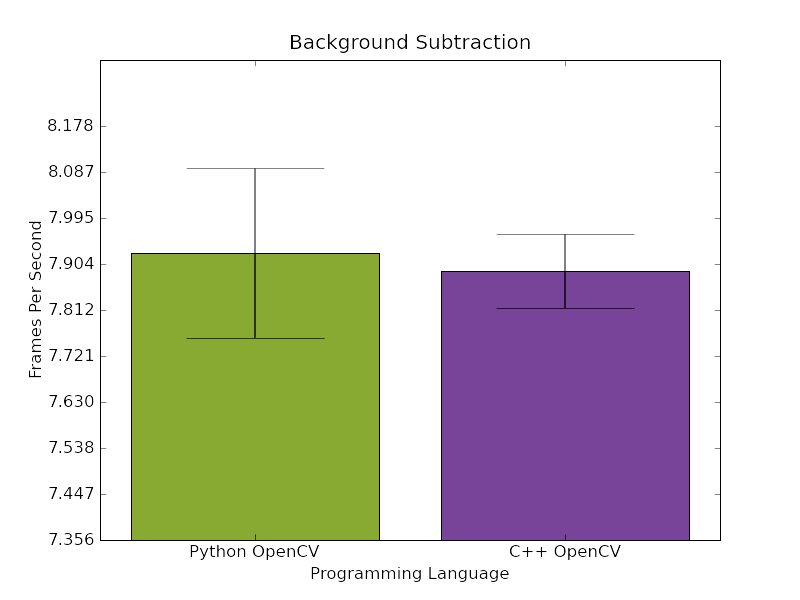
\includegraphics[width=0.95\columnwidth]{report_data/background_subtraction}

\caption{\label{fig:BackgroundSubtract_graph} Background subtraction performances}

\end{figure}


%
\begin{figure}[h]
\subfloat[\label{fig:Adding-a-single}Adding item]{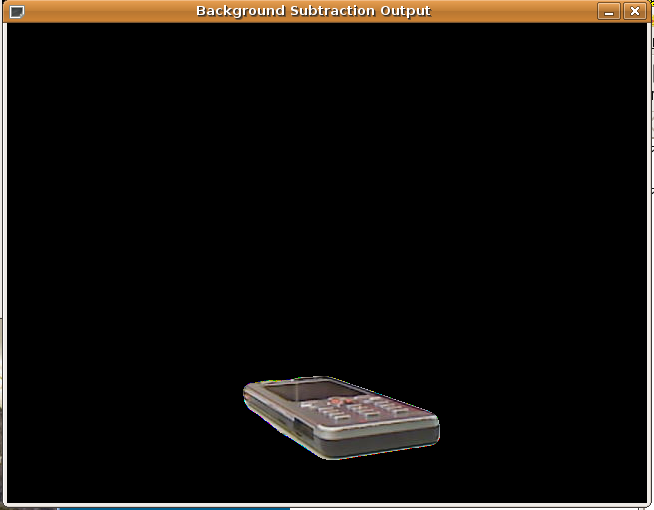
\includegraphics[width=0.33\columnwidth]{report_data/background_python_add_item}}\subfloat[\label{fig:Adding-another-item,}minor problems]{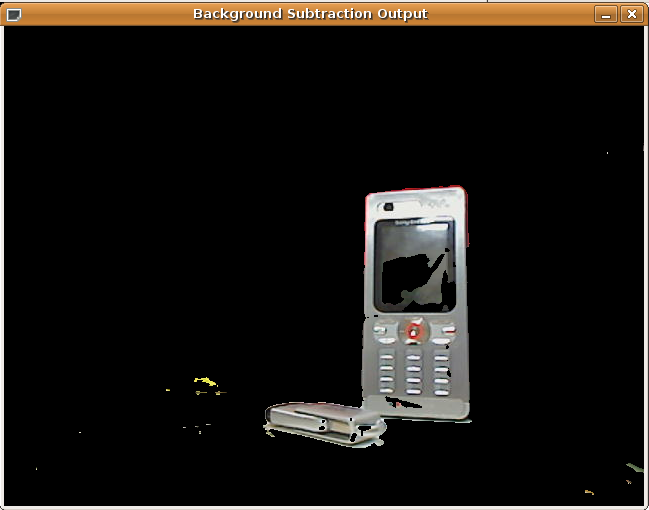
\includegraphics[width=0.33\columnwidth]{report_data/background_python_add_more_items}

}\subfloat[\label{fig:remove-laptop}Addition and removal]{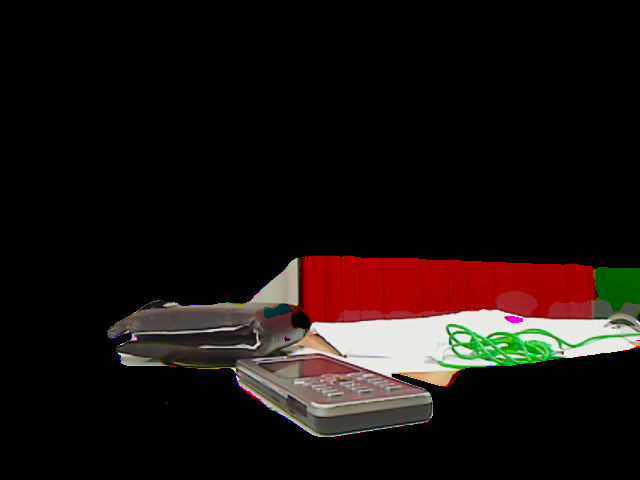
\includegraphics[width=0.33\columnwidth]{report_data/background_python_add_remove_item}

}

\caption{\label{fig:background-Adding-and-removing} Background subtraction
response after adding and removing items from a scene.}

\end{figure}
%
\begin{figure}
\subfloat[before]{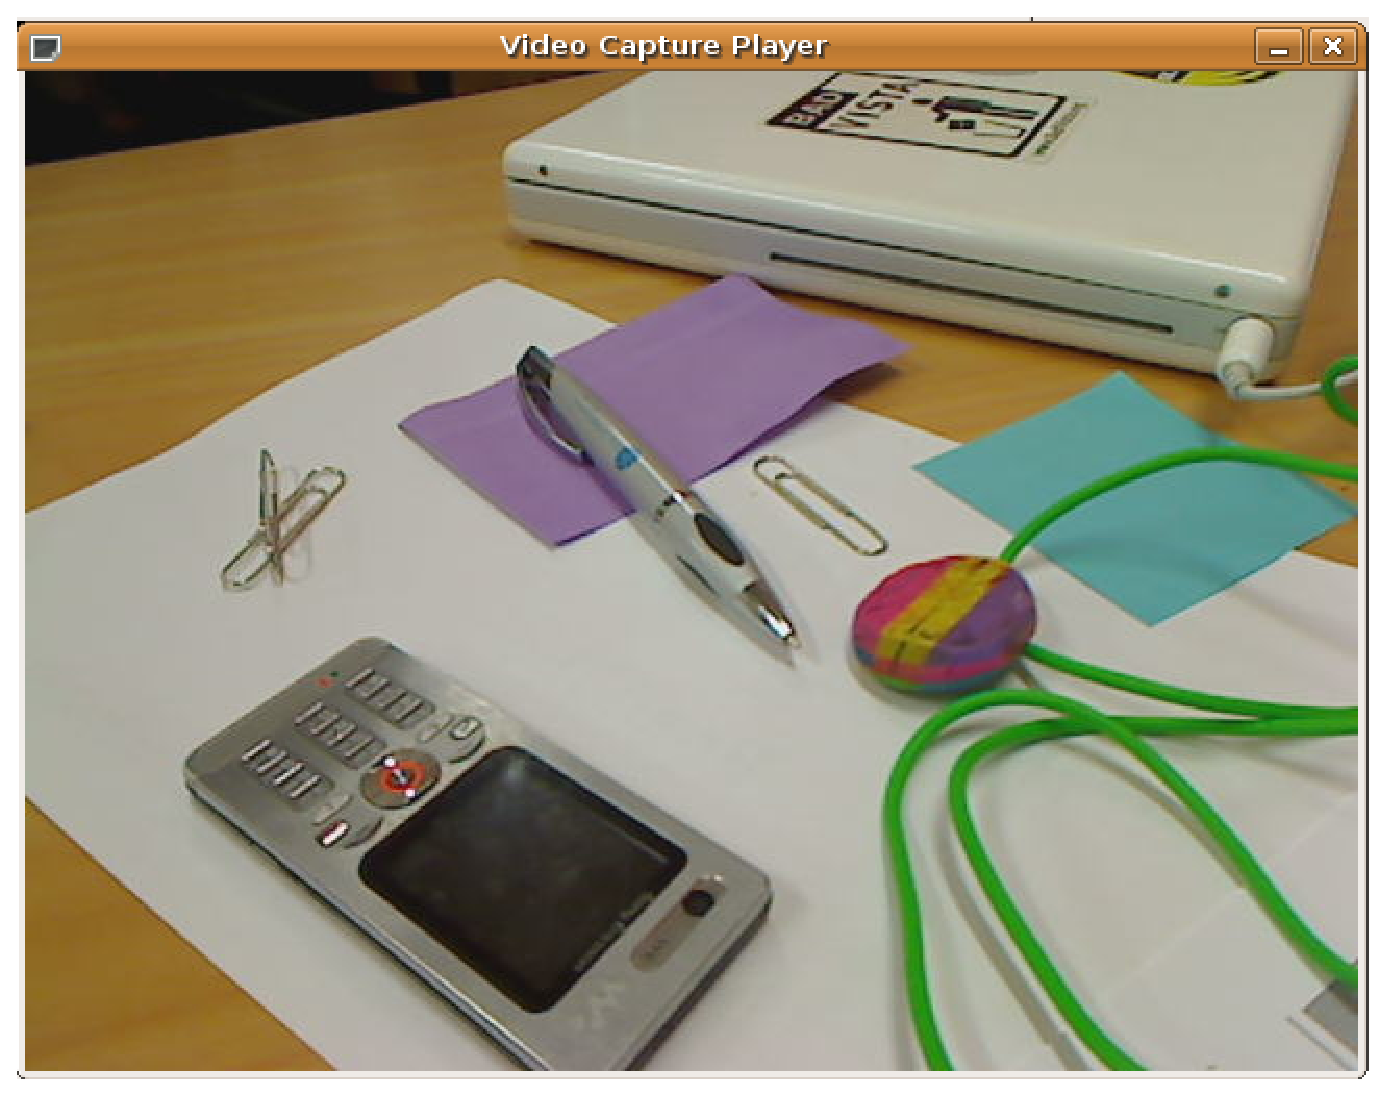
\includegraphics[width=0.3\columnwidth]{report_data/background_python_before}

}\subfloat[program output]{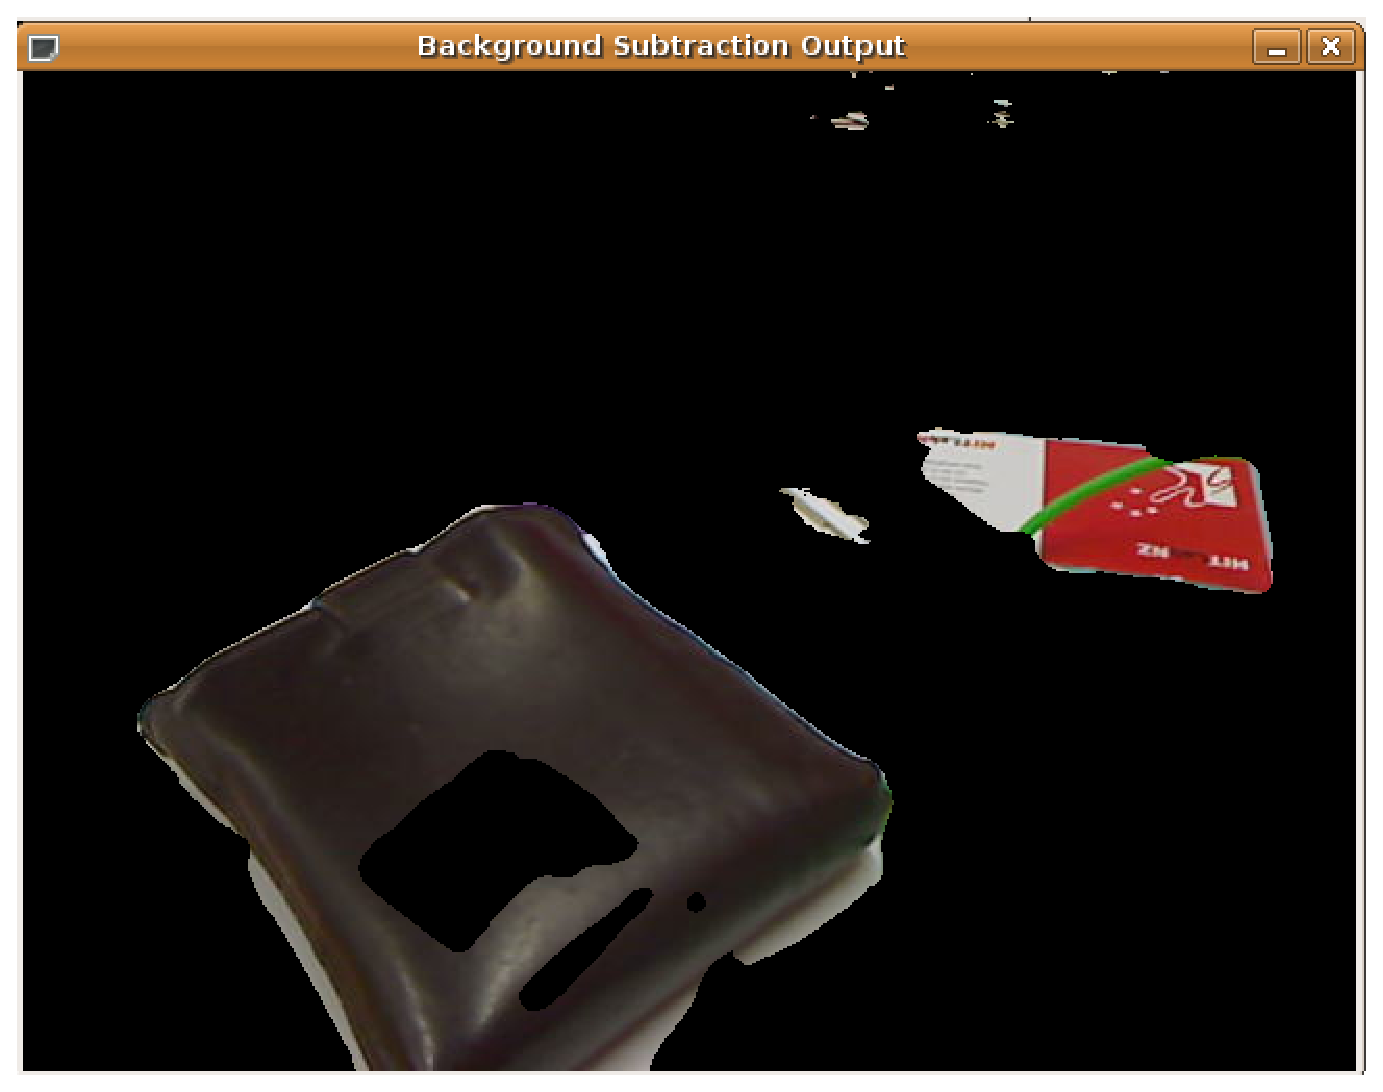
\includegraphics[width=0.3\columnwidth]{report_data/background_python_add_items_complicated}

}\subfloat[after]{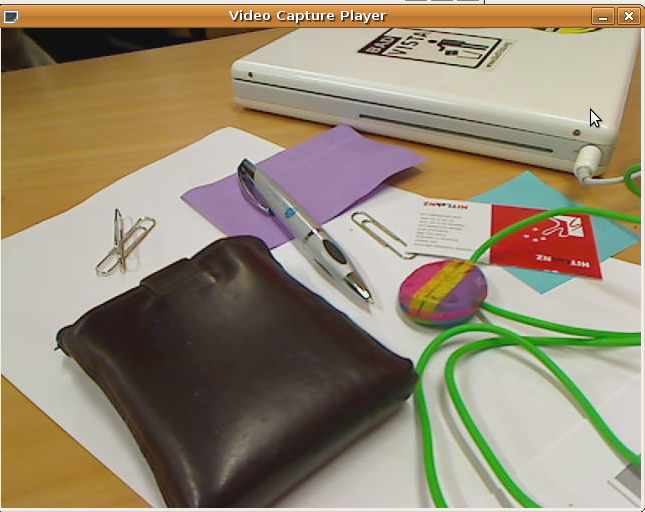
\includegraphics[width=0.3\columnwidth]{report_data/background_python_after}

}

\caption{\label{fig:back-Proces-clutter}Background subtraction response on
a cluttered scene where a cellphone is switched for a wallet and a
contact card is added.}

\end{figure}
 While creating this program, we found IPython particularly helpful,
it allows for interactive, in place trialing, timing and plotting
as shown in algorithm \ref{alg:Interactive,-inplace-timing}.

%
\begin{algorithm}
\noindent In {[}1{]}: from opencv import cv

\noindent In {[}2{]}: cv.cvAnd(diffImage,image, temp)

\noindent In {[}3{]}: timeit cv.cvAnd(diffImage,image, temp)

\noindent 1000 loops, best of 3: 229 \textmu{}s per loop

\noindent In {[}4{]}: from pylab import imshow, show

\noindent In {[}5{]}: imshow(temp) 

\noindent Out{[}5{]}: <AxesImage object at 0x42489d0>

\noindent In {[}6{]}: show()

\caption{\label{alg:Interactive,-inplace-timing}Using IPython, the interactive
shell can be used from deep inside a nested loop in a running program.
In place timing and plotting with access to local variables and functions
like this example speeds up development time.}

\end{algorithm}



\subsection{Feature Point Detection}

Many methods in computer vision for identifying the contents of an
image relies on extracting \emph{interesting} features. An interesting
feature point could be corners of intersecting lines, a line ending,
or any isolated point where local image regions have a high degree
of variation in all directions \cite{harris1988combined}. The features
must be found algorithmically and have a well-defined position. The
repeatability of choosing the same points under differing conditions
is a measure of how good an interesting feature algorithm is. According
to \cite{Sol09} the Harris \& Stephens algorithm is in short: 
\begin{quote}
A matrix W is created from the outer product of the image gradient,
this matrix is averaged over a region and then a corner response function
is defined as the ratio of the determinant to the trace of W.
\end{quote}
A threshold is then applied to this corner response image to pick
the most likely candidates and then these points are plotted. An example
usage of the algorithm is in the Lucas\textendash{}Kanade Optical
Flow Method where it can be used to select good feature points \cite{beauchemin1995computation}
for tracking movement.

%
\begin{figure}[h]
\begin{centering}
\subfloat[\label{fig:harris_scipy_static}SciPy]{\begin{centering}
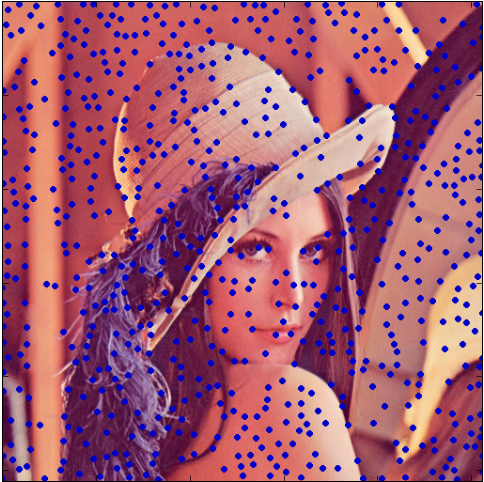
\includegraphics[width=0.45\columnwidth]{harris_scipy_static}
\par\end{centering}

}\subfloat[OpenCV]{\centering{}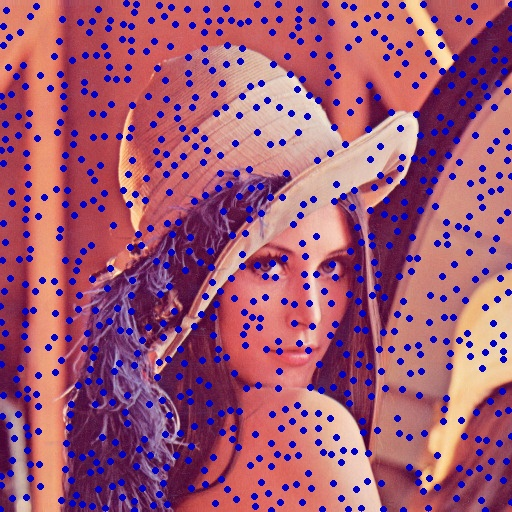
\includegraphics[width=0.45\columnwidth]{harris_response_lena_opencv}}
\par\end{centering}

\caption{\label{fig:harris_compare_static}Running the Harris \& Stephens feature
detection algorithm on the Lena test image.}

\end{figure}
%
%\begin{figure}[h]
%\begin{centering}
%\subfloat[\label{fig:harris_webcam_scipy}SciPy %(\textasciitilde{}4fps)]{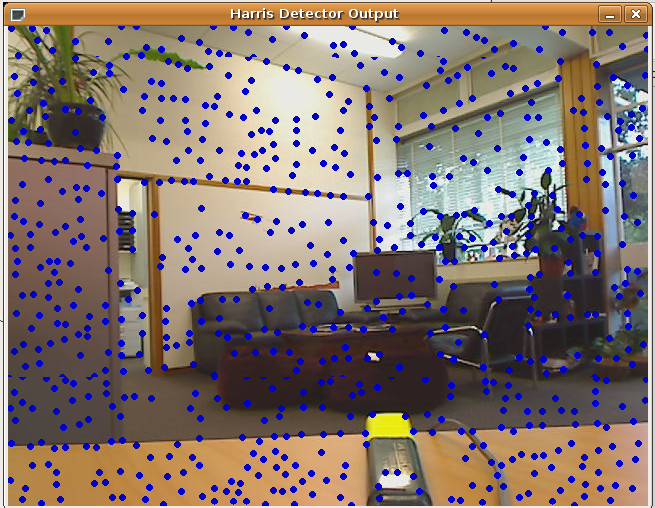
\includegraphics[width=0.45\columnwidth]{report_data/feature_detect/scipy_harris}

%}\subfloat[OpenCV %(\textasciitilde{}9fps)]{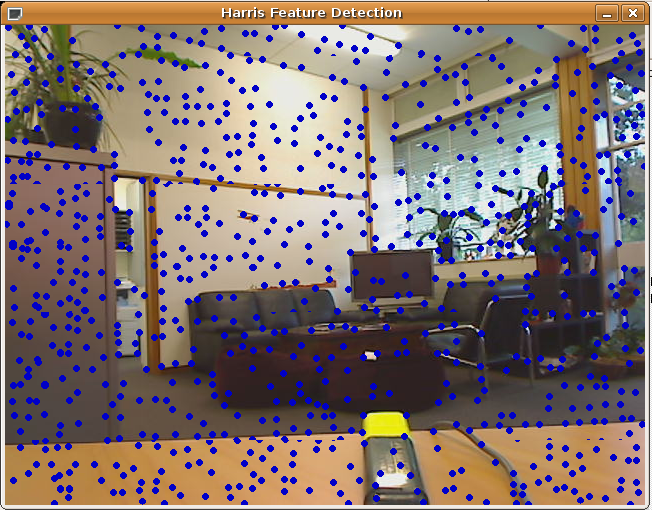
\includegraphics[width=0.45\columnwidth]{report_data/feature_detect/opencv_harris}

%}
%\par\end{centering}

%\caption{\label{fig:harris_compare_webcam}Feature detection running on webcam
%stream}

%\end{figure}


We took and modified an existing implementation in SciPy by \cite{Sol09}
which produced Figures \ref{fig:harris_scipy_static} \& \ref{fig:harris_webcam_scipy}.
The algorithm was timed by executing it on Lena 300 times per sample:

\begin{center}
\begin{tabular}{|c|c|c|}
\hline 
Sample: & Mean & Std\tabularnewline
\hline
\hline 
SciPy & 191.5 ms & 0.87 ms\tabularnewline
\hline 
OpenCV & 65.7 ms & 1.27 ms\tabularnewline
\hline
\end{tabular}
\par\end{center}

The same concept but in a different implementation is shown in Figure
\ref{fig:harris_compare_webcam} for OpenCV. A filter kernel size
of 3 pixels was used when computing the harris response, the authors
did note that with a larger kernel SciPy seemed to slow down more
than OpenCV. The threshold filtering and display of the corner response
was implemented solely in OpenCV to reduce differences; the SciPy
implementation therefore had an extra data conversion stage. Another
limitation is the OpenCV response in C++ is not implemented here.


\subsection{Face Detection}

Face detection is the task of identifying the presence of any number
of faces in an image, this is a specific case of general object detection.
Before locating an object, one must be able to describe it. Many object
detection algorithms use a strong classifier which is built from a
collection of weak feature patterns made by scanning a database of
images with known contents \cite{viola2004robust}. Figure \ref{fig:OpenCV-Face-Detection}
shows the output from our tests running under different conditions
when using the face Haar-cascade classifier that comes with OpenCV.
The method gave an average framerate of 7.16 \textpm{} 0.02 Hz. The
detection process itself gave very consistent timings of 107 \textpm{}
1 ms. The detection method used has limitations as shown in Figures
\ref{fig:Obscured-opencv-face} and \ref{fig:Angled-opencv-face},
this is caused because the classifier was only trained on straight
on face images. But in ideal conditions, with good lighting and un-obscured
faces directly facing the camera the algorithm produces very robust
results. There is no corresponding high level functionality in SciPy,
so a performance comparison was not possible. A recent project PyCV \cite{tri2009principled}
improves on the face detection in OpenCV utilizing SciPy.

%
\begin{figure}[h]
\subfloat[Single face in frame]{\begin{centering}
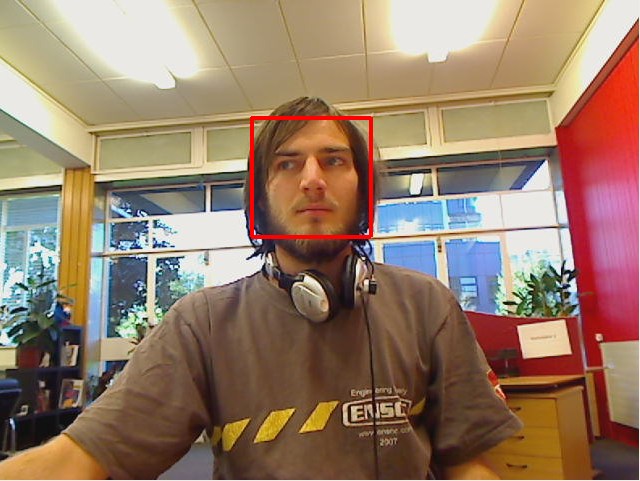
\includegraphics[width=0.45\columnwidth]{report_data/face_detect_one}
\par\end{centering}



}\subfloat[\label{fig:Obscured-opencv-face}Obscured face in frame]{\begin{centering}
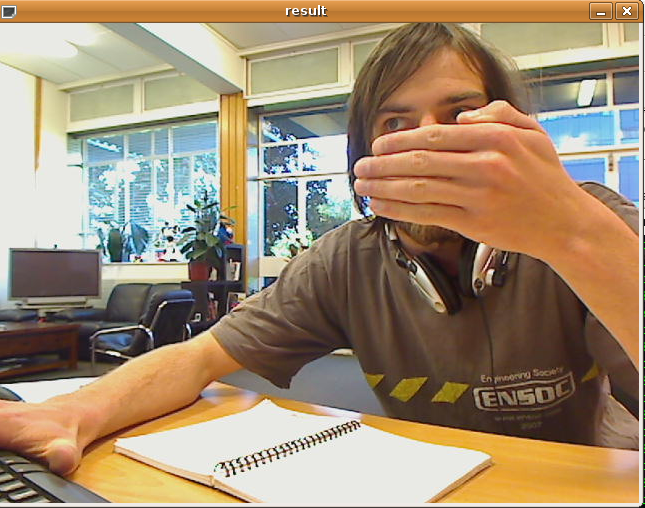
\includegraphics[width=0.45\columnwidth]{report_data/face_detect_obscure}
\par\end{centering}



}

\subfloat[Multiple faces]{\begin{centering}
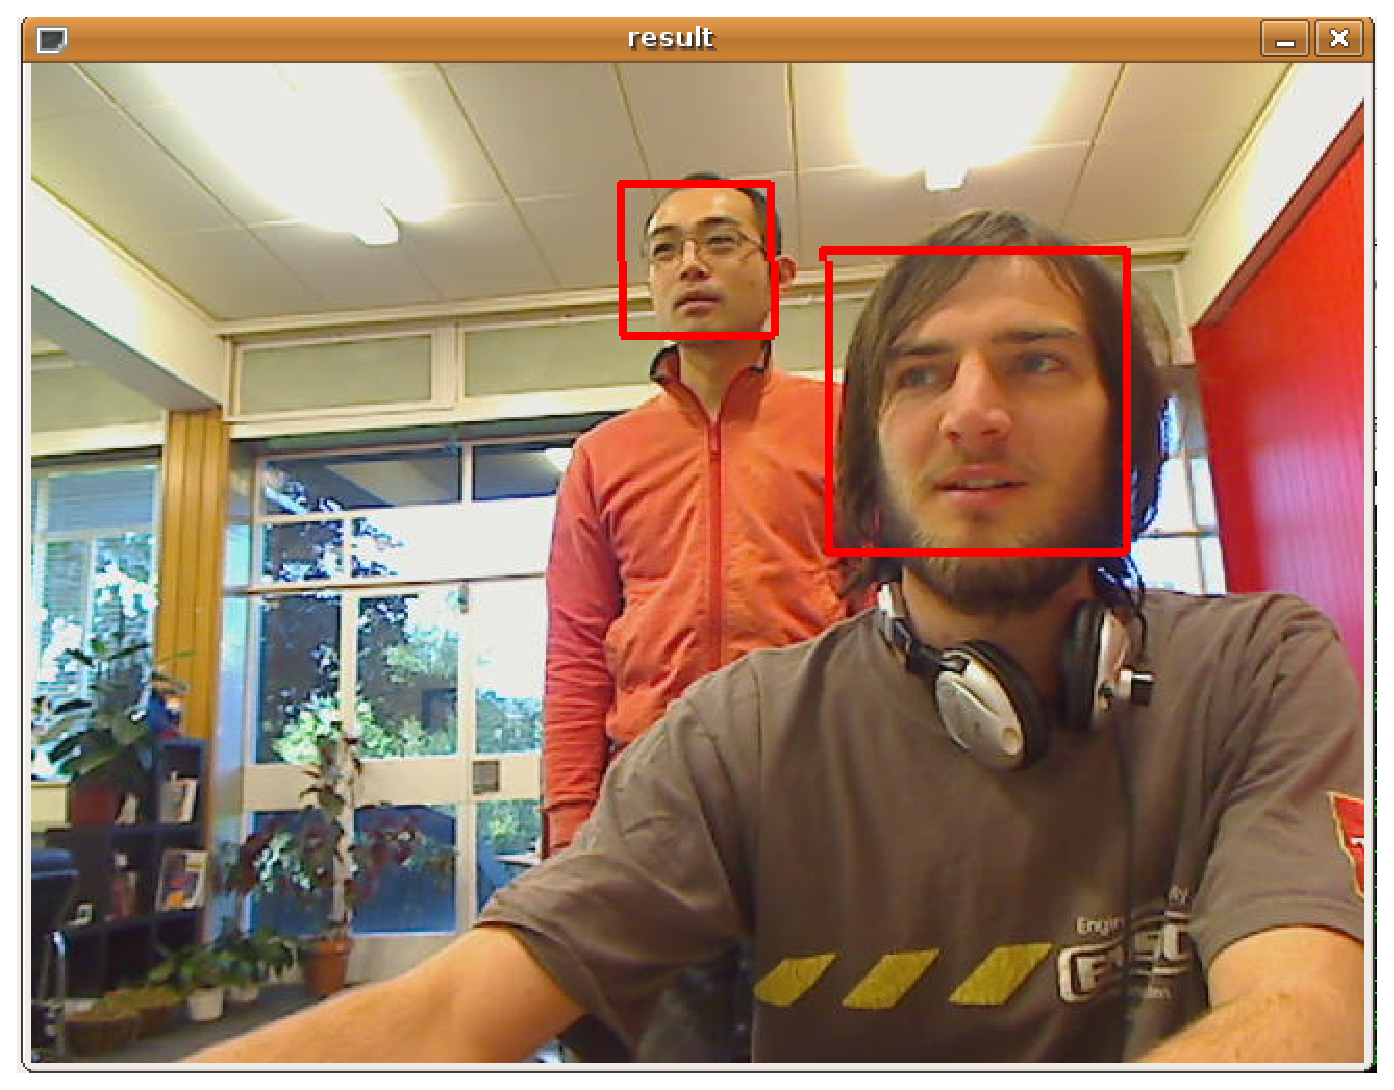
\includegraphics[width=0.45\columnwidth]{report_data/face_detect_two}
\par\end{centering}



}\subfloat[\label{fig:Angled-opencv-face}Rotated face]{\begin{centering}
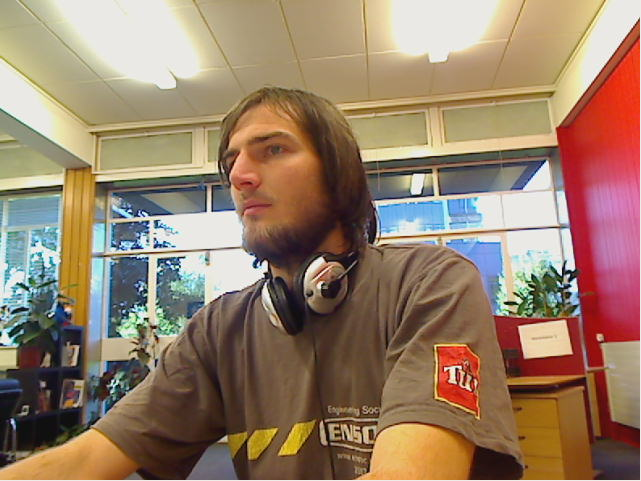
\includegraphics[width=0.45\columnwidth]{report_data/face_detect_sideways}
\par\end{centering}



}

\caption{\label{fig:OpenCV-Face-Detection}OpenCV Face Detection}

\end{figure}


%
\begin{figure}
\begin{centering}
\subfloat[detecting face objects]{\begin{centering}
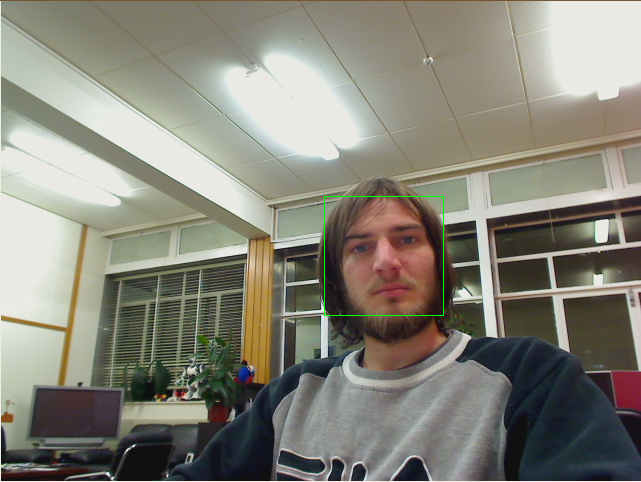
\includegraphics[width=0.45\columnwidth]{report_data/pygame-eye-locate}
\par\end{centering}



}\subfloat[\label{fig:edge-filtering-face}edge filtering and face detection]{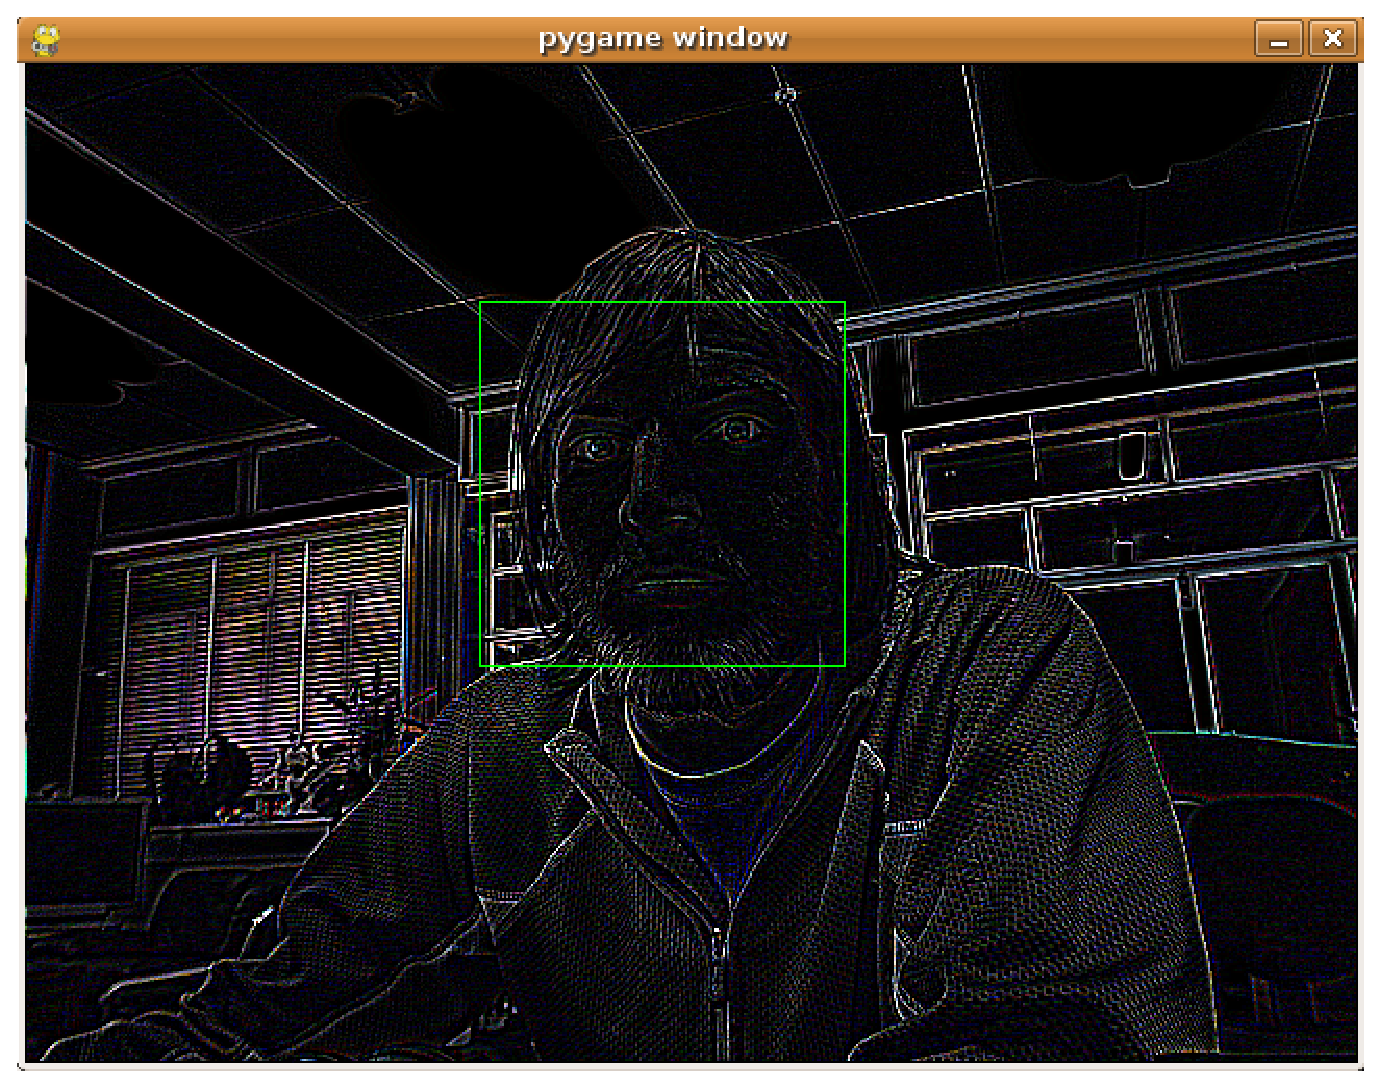
\includegraphics[width=0.45\columnwidth]{report_data/pygame-face-edge}



}
\par\end{centering}

\caption{\label{fig:Pygame-object}Pygame can be used to capture and display
the webcam, while OpenCV does the processing.}



\end{figure}


Figure \ref{fig:Pygame-object} shows an alternative setup; using
the Pygame camera module for image capture, OpenCV for the object
detection and Pygame surfaces for the box rendering and display. Python
really shows its strengths as a glue language here, as the different
libraries are easily used in conjunction with each other. The benefits
from this can be huge, it is very easy for a developer to incorporate
different computer vision tools, even with very limited knowledge
of computer vision. We found that calling OpenCV from a Python wrapper
was only slightly slower in general than natively using the library. 


\section{Qualitative Comparison}

In getting these quantitative results we noticed that the Python implementations
were shorter, easier to create, easier to debug, and easier to test.
Having the use of an interactive interpreter to progressively come
to a solution prototype and being able to use these prototypes in
the final product is a big argument in favor of using Python. 

The documentation in both SciPy and OpenCV was found to be complete,
but not as extensive as for a professional package like Matlab. Support
for these open source packages is almost entirely reliant on experienced
members of the community responding to requests on message boards
or mailing lists. When one of the authors asked a question regarding
the gaussian image filtering function to the SciPy mailing list it
spurred not only an immediate response pointing out the solution to
the direct query but also a discussion on finite approximations to
gaussian kernels, how SciPy and OpenCV might do it differently%
\footnote{One user even went as far as to test and propose a new IIR filter
implementation for SciPy that scales better with kernel size than
the existing implementations.%
}. This kind of support is common in the open source world, where a
package like SciPy prides itself on its very rigorous and open tests. 

For the scholar of computer vision research we find that using Python
can help in trying out new algorithms very quickly. The breadth of
the additional libraries available and the ease of integrating, make
new and novel solutions quickly realizable. 

For those newer to computer vision, we can recommend Python for many
reasons, it is much more forgiving than C or C++, it can be used interactively
so you can happily make 10 mistakes in a row, without having to recompile
and start execution again for each attempted fix.

A major limitation of using Python would be when the application is
being developed for special or embedded hardware or when the best
possible performance is required. The stability of the packages is
also somewhat in question, OpenCV's Python bindings are being rewritten
manually to replace the SWIG produced bindings and SciPy is still
relatively new. In some cases there was no analogous function in both
OpenCV and SciPy. This is because OpenCV is very specific to the CV
domain whereas SciPy is for more general scientific computing.

This graph was created interactively using the Python plotting package
Matplotlib from IPython acting directly on the data from OpenCV. With
just two lines of Python code, which can be put anywhere in a computer
vision program, we can pause execution and drop into a live interactive
shell with full plotting capabilities. {}``\emph{from IPython.Shell
import IPShellEmbed}'' and {}``\emph{IPShellEmbed()()}'' This means
that as developers, to debug a misbehaving program, we can just jump
right into the middle of a deeply nested loop, introspect all variables,
plot any signal or image, call any function, and accurately time the
execution of any function. This is massively in favor of using Python.

\section{Related Works}

A feature of SciPy that has previously gone unmentioned, is the Weave
module for in-lining C and C++ code. This can produce code 100x faster \cite{ramachandran-performance}
than pure Python. As mentioned in the introduction many CV algorithms
are currently developed using Matlab, the tool \noun{OMPC} has been
created for compiling Matlab into Python\cite{jurica2009ompc}.

For parallel programming, mixed language solutions have been shown
to exhibit the same performance gains as native language solutions \cite{cai2005performance}.
A different direction for parallel solutions is to harness the power
of the graphics card many desktop computers have, the PyGPU and the
GPUCV projects both allow leveraging this technology from Python \cite{lejdfors2006implementing} \cite{farrugia2006gpucv} \cite{allusse2008gpucv}.

Another related area of research is the performance of Python itself.
One such project was the Psyco \emph{just in time compiler} for Python \cite{rigo2004representation},
unfortunately Psyco only works on Python 2.6.X and on x86 machines.
The developer of Psyco is currently working on the performance of
PyPy \cite{dubois2005nest}, a compliant, flexible and fast implementation
of the Python Language. Google is currently midway through their \noun{Unladen
Swallow} project which aims to speed up Python by leveraging the \noun{Low
Level Virtual Machine} (LLVM). All of these projects help make Python
a safe bet for the future of scientific computing and specifically
for use in the computer vision domain. Pyro \cite{blank2003pyro} is
a robotics simulation environment that including computer vision modules.


\subsection*{Acknowledgments}

Thanks to all the developers that invest their own valuable time to
work on open source projects OpenCV, Python and SciPy.

\bibliographystyle{ieeetr}
\bibliography{report_data/database}

\end{document}
